%%%%%%%%%%%%%%%%%%%%%%%%%%%%%%%%%%%%%%%%%%%%%%%%%%%%%%%%%%%%%%%%%%%%%%%%%%%%%%%%%%
\begin{frame}[fragile]\frametitle{}

\begin{center}
{\Large Parts of Speech}
\end{center}
\end{frame}

%%%%%%%%%%%%%%%%%%%%%%%%%%%%%%%%%%%%%%%%%%%%%%%%%%%%%%%%%%%%%%%%%%%%%%%%%%%%%%%%%%
\begin{frame}[fragile]\frametitle{Terminology}

  \begin{itemize}
  \item Tagging: The process of associating labels with each token in a text
  \item Tags: The labels, Syntactic word classes
  \item Tag Set: The collection of tags used
  \end{itemize}
\end{frame}

%%%%%%%%%%%%%%%%%%%%%%%%%%%%%%%%%%%%%%%%%%%%%%%%%%%%%%%%%%%%%%%%%%%%%%%%%%%%%%%%%%
\begin{frame}[fragile]\frametitle{Parts of speech}

  \begin{itemize}
  \item How can we predict the bahaviour of a unseen word?
  \item Words can be divided into classes that behave similarly.
  \item Traditionally eight parts of speech: noun, verb,
    pronoun, preposition, adverb, conjunction, adjective and article.
  \item More recently larger sets have been used: eg Penn Treebank (45
    tags), Susanne (353 tags).
  \end{itemize}
\end{frame}

%%%%%%%%%%%%%%%%%%%%%%%%%%%%%%%%%%%%%%%%%%%%%%%%%%%%%%%%%%%%%%%%%%%%%%%%%%%%%%%%%%
\begin{frame}[fragile]\frametitle{Parts of speech}
  Eight major parts of speech for words are: 
  \begin{itemize}

  \item Noun: people, animals, concepts, things (e.g. ``birds'')
  \item Pronoun: a word used in place of a noun (e.g. ``it'', ``they'', ``I'', ``she'')
  \item Verb: express action in the sentence (e.g. ``sing'')
  \item Adjective: describe properties of nouns (e.g. ``yellow'')
  \item Adverb: modifies or describes a verb, an adjective, or another adverb (e.g. ``extremely'', ``slowly'')
  \item Preposition: a word placed before a noun/pronoun to form a phrase modifying another word/phrase (e.g. ``in'', ``for'', ``without'')
  \item Conjunction: a word that connects/conjoins another sentence or phrase (e.g. ``and'', ``or'', ``but'', ``so'', ``Since'') 
  \item Interjection: a word that expresses spontaneous feeling (e.g. ``uh'').

 
  \end{itemize}
\end{frame}


%%%%%%%%%%%%%%%%%%%%%%%%%%%%%%%%%%%%%%%%%%%%%%%%%%%%%%%%%%%%%%%%%%%%%%%%%%%%%%%%%%
\begin{frame}[fragile]\frametitle{Parts of Speech}

  \begin{alertblock}{What use are parts of speech?}
    They tell us a lot about a word (and the words near it).
  \end{alertblock}

  
  \begin{itemize}
  \item Tell us what words are likely to occur in the neighbourhood
    (eg adjectives often followed by nouns, personal pronouns often
    followed by verbs, possessive pronouns by nouns)
  \item Pronunciations can be dependent on part of speech, eg
    \textcolor{green}{object, content, discount} (useful for speech
    synthesis and speech recognition)
  \item Can help information retrieval and extraction (stemming,
    partial parsing) 
  \item Useful component in many NLP systems
  \end{itemize}
  
\end{frame}

%%%%%%%%%%%%%%%%%%%%%%%%%%%%%%%%%%%%%%%%%%%%%%%%%%%%%%%%%%%%%%%%%%%%%%%%%%%%%%%%%%
\begin{frame}[fragile]\frametitle{Closed and open classes}
  \begin{itemize}
  \item Parts of speech may be categorised as \emph{open} or
    \emph{closed} classes
  \item Closed classes have a fixed membership of words (more or
    less), eg determiners, pronouns, prepositions
  \item Closed class words are usually \emph{function words} ---
    frequently occurring, grammatically important, often short (eg
    \textcolor{green}{of,it,the,in})
  \item The major open classes are \emph{nouns}, \emph{verbs},
    \emph{adjectives} and \emph{adverbs}
  \end{itemize}
\end{frame}

%%%%%%%%%%%%%%%%%%%%%%%%%%%%%%%%%%%%%%%%%%%%%%%%%%%%%%%%%%%%%%%%%%%%%%%%%%%%%%%%%%
\begin{frame}[fragile]\frametitle{Closed classes in English}
  \textcolor{black}{
  \begin{tabular}{ll}
  \textbf{prepositions} & on, under, over, to, with, by\\
  \textbf{determiners} & the, a, an, some\\
  \textbf{pronouns} & she, you, I, who\\
  \textbf{conjunction}s & and, but, or, as, when, if\\
  \textbf{auxiliary verbs} & can, may, are\\
  \textbf{particles} & up, down, at, by\\
  \textbf{numeral}s & one, two, first, second\\
  \end{tabular}}
\end{frame}

%%%%%%%%%%%%%%%%%%%%%%%%%%%%%%%%%%%%%%%%%%%%%%%%%%%%%%%%%%%%%%%%%%%%%%%%%%%%%%%%%%
\begin{frame}[fragile]\frametitle{Open classes}
  \textcolor{black}{
  \begin{description}
  \item[nouns] Proper nouns (\textcolor{green}{Scotland}, \textcolor{green}{BBC}),\\
    common nouns:
    \begin{itemize}
    \item count nouns (\textcolor{green}{goat},
      \textcolor{green}{glass})
    \item mass nouns (\textcolor{green}{snow},
      \textcolor{green}{pacifism})
    \end{itemize}
  \item[verbs] actions and processes (\textcolor{green}{run},
    \textcolor{green}{hope}), also auxiliary verbs
  \item[adjectives] properties and qualities (age, colour, value)
  \item[adverbs] modify verbs, or verb phrases, or other adverbs:\\
    \textcolor{green}{\emph{Unfortunately} John walked \emph{home
        extremely slowly yesterday}}
  \end{description}}
\end{frame}


%%%%%%%%%%%%%%%%%%%%%%%%%%%%%%%%%%%%%%%%%%%%%%%%%%%%%%%%%%%%%%%%%%%%%%%%%%%%%%%%%%
\begin{frame}[fragile]\frametitle{The Penn Treebank tagset (1)}
  \textcolor{black}{\footnotesize
    \begin{tabular}{|lll|lll|}
      \hline
      CC & Coord Conjuncn & \emph{and,but,or} &  
      NN & Noun, sing. or mass & \emph{dog} \\
      CD & Cardinal number & \emph{one,two} & 
      NNS & Noun, plural & \emph{dogs} \\
      DT & Determiner & \emph{the,some} &  
      NNP & Proper noun, sing. & \emph{Edinburgh} \\
      EX & Existential there & \emph{there} &  
      NNPS & Proper noun, plural & \emph{Orkneys} \\
      FW & Foreign Word & \emph{mon dieu} &  
      PDT & Predeterminer & \emph{all, both}\\
      IN & Preposition & \emph{of,in,by} & 
      POS & Possessive ending & \emph{'s} \\
      JJ & Adjective & \emph{big} & 
      PP & Personal pronoun & \emph{I,you,she} \\
      JJR & Adj., comparative & \emph{bigger} & 
      PP\$ & Possessive pronoun & \emph{my,one's} \\
      JJS & Adj., superlative & \emph{biggest} &  
      RB & Adverb & \emph{quickly} \\
      LS & List item marker & \emph{1,One} &  
      RBR & Adverb, comparative & \emph{faster} \\
      MD & Modal & \emph{can,should} &
      RBS & Adverb, superlative & \emph{fastest} \\
      \hline
    \end{tabular}
  }
\end{frame}

%%%%%%%%%%%%%%%%%%%%%%%%%%%%%%%%%%%%%%%%%%%%%%%%%%%%%%%%%%%%%%%%%%%%%%%%%%%%%%%%%%
\begin{frame}[fragile]\frametitle{The Penn Treebank tagset (2)}
  \textcolor{black}{\footnotesize
    \begin{tabular}{|lll|lll|}
      \hline
      RP & Particle & \emph{up,off} &
      WP\$ & Possessive-Wh & \emph{whose} \\ 
      SYM & Symbol & \emph{+,\%,\&}  &
      WRB & Wh-adverb & \emph{how,where} \\
      TO & ``to'' & \emph{to} &
      \$ & Dollar sign & \emph{\$}\\
      UH & Interjection & \emph{oh, oops} &
      \# & Pound sign & \emph{\#} \\
      VB & verb, base form &     \emph{eat} &
      `` & Left quote & ` , `` \\
      VBD & verb, past tense & \emph{ate} &
      '' & Right quote & ', '' \\
      VBG & verb, gerund & \emph{eating} &
      ( & Left paren & ( \\
      VBN & verb, past part & \emph{eaten} &
      ) & Right paren & ) \\
      VBP & Verb, non-3sg, pres & \emph{eat} &
      , & Comma & , \\
      VBZ & Verb, 3sg, pres & \emph{eats} &
      . & Sent-final punct & . ! ? \\
      WDT & Wh-determiner &  \emph{which,that} &
      : & Mid-sent punct. & : ; --- ... \\
      WP & Wh-pronoun & \emph{what,who} & & & \\
      \hline
    \end{tabular}
  }
\end{frame}

%%%%%%%%%%%%%%%%%%%%%%%%%%%%%%%%%%%%%%%%%%%%%%%%%%%%%%%%%%%%%%%%%%%%%%%%%%%%%%%%%%
\begin{frame}[fragile]\frametitle{Part-of-Speech Ambiguity}

\begin{center}
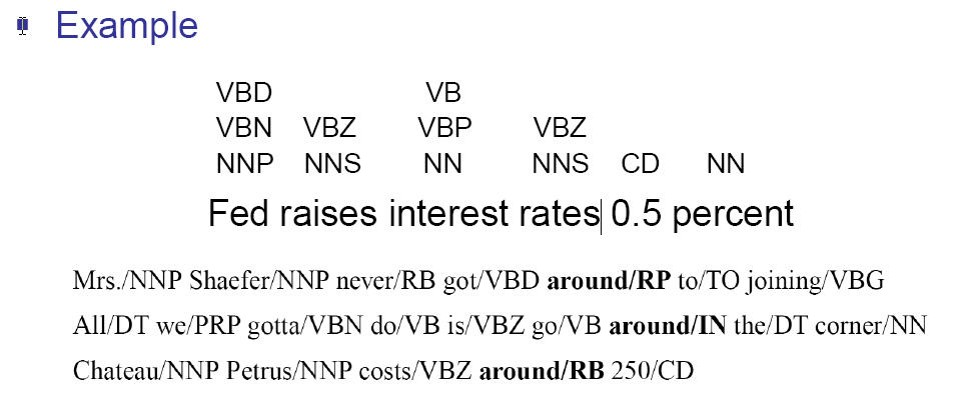
\includegraphics[width=\linewidth,keepaspectratio]{pos1}
\end{center}
  
\end{frame}


%%%%%%%%%%%%%%%%%%%%%%%%%%%%%%%%%%%%%%%%%%%%%%%%%%%%%%%%%%%%%%%%%%%%%%%%%%%%%%%%%%
\begin{frame}[fragile]\frametitle{Sources  of information}
  \begin{itemize}
  \item Syntagmatic: tags of the other words:
    \begin{itemize}
  \item AT JJ NN is common
  \item AT JJ VBP impossible (or unlikely)
    \end{itemize}
  \item Lexical: look at the words
    \begin{itemize}
  \item The : AT
  \item Flour : more likely to be a noun than a verb
  \item A tagger that always chooses the most common tag is 90\% correct (often used as baseline)
    \end{itemize}
  \item Most taggers use both 
  \end{itemize}
\end{frame}

%%%%%%%%%%%%%%%%%%%%%%%%%%%%%%%%%%%%%%%%%%%%%%%%%%%%%%%%%%%%%%%%%%%%%%%%%%%%%%%%%%
\begin{frame}[fragile]\frametitle{What does Tagging do?}
  \begin{itemize}
  \item Collapses Distinctions: Lexical identity may be discarded e.g., all personal pronouns tagged with PRP
  \item Introduces Distinctions: Ambiguities may be resolved e.g. deal tagged with NN or VB
   \item Helps in classification and prediction
  \end{itemize}
\end{frame}


%%%%%%%%%%%%%%%%%%%%%%%%%%%%%%%%%%%%%%%%%%%%%%%%%%%%%%%%%%%%%%%%%%%%%%%%%%%%%%%%%%
\begin{frame}[fragile]\frametitle{Tagging}
  \begin{itemize}
  \item Definition: POS Tagging is the assignment of a single
    part-of-speech tag to each word (and punctuation marker) in a
    corpus.  For example:\\
    {\scriptsize
    \textcolor{green}{``/``  The/DT  guys/NNS  that/WDT  make/VBP
      traditional/JJ  hardware/NN  are/VBP  really/RB  being/VBG
      obsoleted/VBN  by/IN  microprocessor-based/JJ  machines/NNS  ,/,
      ''/''  said/VBD  Mr./NNP  Benton/NNP  ./.}}
  \item Non-trivial: POS tagging must resolve ambiguities since the
    same word can have different tags in different contexts
  \item In the Brown corpus 11.5\% of word types and 40\% of word
    tokens are ambiguous
  \item In many cases one tag is much more likely for a given word
    than any other
  \item Limited scope: only supplying a tag for each word, no larger
    structures created (eg prepositional phrase attachment)
  \end{itemize}  
\end{frame}

%There                  EX
%are                    VBP
%11                     CD
%players                        NNS
%in                     IN
%a                      DT
%football               NN
%team                   NN
%.                      .

%%%%%%%%%%%%%%%%%%%%%%%%%%%%%%%%%%%%%%%%%%%%%%%%%%%%%%%%%%%%%%%%%%%%%%%%%%%%%%%%%%
\begin{frame}[fragile]\frametitle{Information sources for tagging}
  \textcolor{black}{
  What information can help decide the correct PoS tag for a word?
  \begin{description}
  \item[Other PoS tags] Even though the PoS tags of other words may be
    uncertain too, we can use information that some tag sequences are
    more likely than others (eg \emph{the/AT red/JJ drink/NN} vs \emph{the/AT
      red/JJ drink/VBP}).\newline
    Using \emph{only} information about the most likely PoS tag
    sequence does not result in an accurate tagger (about 77\%
    correct)
  \item[The word identity] Many words can gave multiple possible tags,
    but some are more likely than others (eg \emph{fall/VBP} vs
    \emph{fall/NN}) \newline
    Tagging each word with its most common tag results in a tagger
    with about 90\% accuracy
  \end{description}}
\end{frame}

%%%%%%%%%%%%%%%%%%%%%%%%%%%%%%%%%%%%%%%%%%%%%%%%%%%%%%%%%%%%%%%%%%%%%%%%%%%%%%%%%%
\begin{frame}[fragile]\frametitle{Tagging methods}
  \begin{itemize}
  \item Hand-coded
  \item Statistical taggers: N-Gram Tagging, HMM, (Maximum Entropy)
  \item Brill (transformation-based) tagger
  \end{itemize}
\end{frame}

%%%%%%%%%%%%%%%%%%%%%%%%%%%%%%%%%%%%%%%%%%%%%%%%%%%%%%%%%%%%%%%%%%%%%%%%%%%%%%%%%%
\begin{frame}[fragile]\frametitle{Hand-coded Tagger}
The Regular Expression Tagger 

\begin{center}
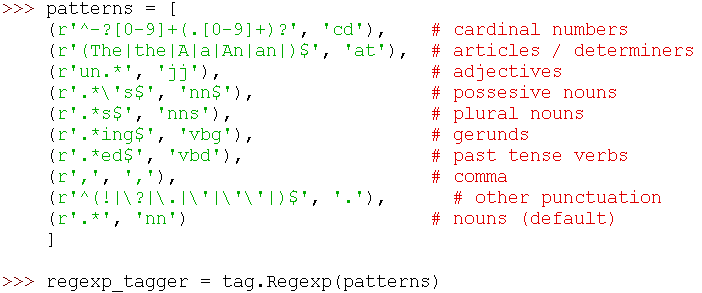
\includegraphics[width=\linewidth,keepaspectratio]{pos3}
\end{center}
  
\end{frame}

%%%%%%%%%%%%%%%%%%%%%%%%%%%%%%%%%%%%%%%%%%%%%%%%%%%%%%%%%%%%%%%%%%%%%%%%%%%%%%%%%%
\begin{frame}[fragile]\frametitle{Unigram Tagger}
  \begin{itemize}
  \item We train a UnigramTagger by specifying tagged sentence data as a parameter when we initialize the tagger.
  \item The training process involves inspecting the tag of each word and storing the most likely tag for any word in a dictionary, stored inside the tagger.
  \end{itemize}

\begin{center}
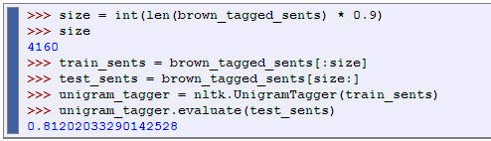
\includegraphics[width=0.5\linewidth,keepaspectratio]{pos4}
\end{center}
  
\end{frame}


%%%%%%%%%%%%%%%%%%%%%%%%%%%%%%%%%%%%%%%%%%%%%%%%%%%%%%%%%%%%%%%%%%%%%%%%%%%%%%%%%%
\begin{frame}[fragile]\frametitle{Error analysis}
  \begin{itemize}
  \item The \% correct score doesn't tell you everything --- it is
    useful know what is misclassified as what
  \item \emph{Confusion matrix}: A matrix (ntags x ntags) where the rows
    correspond to the correct tags and the columns correspond to the
    tagger output.  Cell $(i,j)$ gives the count of the number of
    times tag $i$ was classified as tag $j$
  \item The leading diagonal elements correspond to correct
    classifications
  \item Off diagonal elements correspond to misclassifications 
  \item Thus a confusion matrix gives information on the major
    problems facing a tagger (eg NNP vs. NN vs. JJ)
%  \item See section 3 of the NLTK tutorial on Tagging
  \end{itemize}
\end{frame}

%%%%%%%%%%%%%%%%%%%%%%%%%%%%%%%%%%%%%%%%%%%%%%%%%%%%%%%%%%%%%%%%%%%%%%%%%%%%%%%%%%

\begin{frame}[fragile]\frametitle{N-gram taggers}
  \begin{itemize}
  \item Basic idea:  Choose the tag  that maximises:
    \[ P(\mbox{word} | \mbox{tag}) \cdot 
       P(\mbox{tag} | \mbox{previous n tags}) \]
       
  \item For a bigram model the best tag at position $i$ is:
    \[ t_i = \arg\max_{t_j} P(w_i|t_j) P(t_j | t_{i-1}) \]
    Assuming that you know the previous tag, $t_{i-1}$.
  \item Interpretation: choose the tag $t_i$ that is most likely to
    \alert{generate} word $w_i$ given that the previous tag was $t_{i-1}$ 
  \end{itemize}
\end{frame}

%%%%%%%%%%%%%%%%%%%%%%%%%%%%%%%%%%%%%%%%%%%%%%%%%%%%%%%%%%%%%%%%%%%%%%%%%%%%%%%%%%
\begin{frame}[fragile]\frametitle{N-gram taggers}
\begin{center}
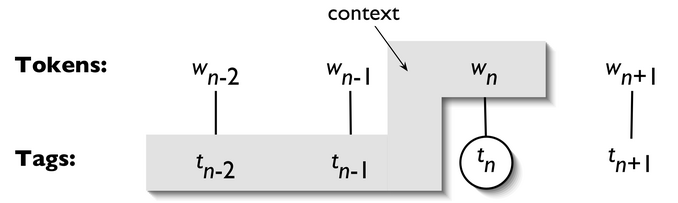
\includegraphics[width=\linewidth,keepaspectratio]{tag-context}
\end{center}
\end{frame}

%%%%%%%%%%%%%%%%%%%%%%%%%%%%%%%%%%%%%%%%%%%%%%%%%%%%%%%%%%%%%%%%%%%%%%%%%%%%%%%%%%
\begin{frame}[fragile]\frametitle{Example (J+M, p304)}
  {\small
  Secretariat/NNP is/VBZ expected/VBZ to/TO \alert{race/VB} tomorrow/NN

  \medskip
  People/NNS continue/VBP to/TO inquire/VB the/DT reason/NN for/IN the/DT
  \alert{race/NN} for/IN outer/JJ space/NN
  }

  \begin{itemize}
  \item``race'' is a verb in the first, a noun in the second.
  \item Assume that race is the only untagged word, so we can assume
    the tags of the others.
  \item Probabilities of ``race'' being a verb, or race being a noun
    in the first example:
    \begin{align*}
      P(\mbox{race is }VB) &= P(VB|TO) P(\mbox{race}|VB) \\
      P(\mbox{race is }NN) &= P(NN|TO) P(\mbox{race}|NN) 
    \end{align*}
  \end{itemize}
\end{frame}

%%%%%%%%%%%%%%%%%%%%%%%%%%%%%%%%%%%%%%%%%%%%%%%%%%%%%%%%%%%%%%%%%%%%%%%%%%%%%%%%%%
\begin{frame}[fragile]\frametitle{Example (continued)}
  \begin{align*}
    P(NN|TO) &= 0.021 \\
    P(VB|TO) &= 0.34 \\
    \\
    P(\mbox{race}|NN) &= 0.00041\\
    P(\mbox{race}|VB) &= 0.00003\\
    \\
    P(\mbox{race is }VB) &= P(VB|TO) P(\mbox{race}|VB) \\
    &= 0.34 \times 0.00003 = 0.00001 \\
    P(\mbox{race is }NN) &= P(NN|TO) P(\mbox{race}|NN) \\
    &= 0.021 \times 0.00041 = 0.000007
   \end{align*}
\end{frame}

%%%%%%%%%%%%%%%%%%%%%%%%%%%%%%%%%%%%%%%%%%%%%%%%%%%%%%%%%%%%%%%%%%%%%%%%%%%%%%%%%
\begin{frame}[fragile]\frametitle{Limitation of NLTK n-gram taggers}

  \begin{itemize}
  \item Does not find the most likely sequence of tags, simply works
    left to right always assigning the most probable single tag (given
    the previous tag assignments)
  \item Does not cope with zero probability problem well (no smoothing
    or discounting)
  \item see module \verb|nltk.tag.hmm|
  \end{itemize}
\end{frame}

%%%%%%%%%%%%%%%%%%%%%%%%%%%%%%%%%%%%%%%%%%%%%%%%%%%%%%%%%%%%%%%%%%%%%%%%%%%%%%%%%%%
%\begin{frame}[fragile]\frametitle{Brill Tagger}
%  \begin{itemize}
%  \item Problem with n-gram taggers: size
%  \item A rule-based system...
%  \item ...but the rules are learned from a corpus
%  \item Basic approach: start by applying general rules, then
%    successively refine with additional rules that correct the
%    mistakes (painting analogy)
%  \item Learn the rules from a corpus, using a set of rule templates,
%    eg:\\
%    Change tag \textbf{a} to \textbf{b} when the following word is
%    tagged \textbf{z}
%  \item Choose the best rule each iteration    
%  \end{itemize}
%\end{frame}
%
%%%%%%%%%%%%%%%%%%%%%%%%%%%%%%%%%%%%%%%%%%%%%%%%%%%%%%%%%%%%%%%%%%%%%%%%%%%%%%%%%%%
%\begin{frame}[fragile]\frametitle{Brill Tagger: Example}
%{\scriptsize
%RNNVB : Replace \texttt{NN} with \texttt{VB} when the previous word is \texttt{TO}\\
%RTOIN: Replace \texttt{TO} with \texttt{IN} when the next tag is \texttt{nns}\\
%\begin{tabular}{lllll} \hline
%\textbf{Sentence}
%& \textbf{Gold}
%& \textbf{Unigram}
%& \textbf{RNNVB}
%& \textbf{RTOIN} \\\hline
%The            & AT      & AT \\
%President      & NN-TL   & NN-TL \\
%said           & VBD     & VBD \\
%he             & PPS     & PPS \\
%will           & MD      & MD \\
%ask            & VB      & VB \\
%Congress       & NP      & NP \\
%to             & TO      & TO \\
%increase       & VB      & \textit{NN}     &    \textit{VB} \\
%grants         & NNS     & NNS \\
%to             & IN      & \textit{TO}     &    \textit{TO} &   \textit{IN} \\
%states         & NNS     & NNS \\
%for            & IN      & IN \\
%vocational     & JJ      & JJ \\
%rehabilitation & NN      & NN
%\end{tabular}
%}
%\end{frame}

%%%%%%%%%%%%%%%%%%%%%%%%%%%%%%%%%%%%%%%%%%%%%%%%%%%%%%%%%%%%%%%%%%%%%%%%%%%%%%%%%%
\begin{frame}[fragile]\frametitle{Summary}
  \begin{itemize}
%  \item \textbf{Reading:} 
%    Jurafsky and Martin, chapter 8 (esp. sec 8.5); 
%    Manning and Sch\"utze, chapter 10; 
  \item Rule-based and statistical tagging
  \item HMMs and n-grams for statistical tagging
  \item Operation of a simple bigram tagger
%  \item TnT --- an accurate trigram-based tagger
  \end{itemize}
\end{frame}
